\documentclass[aspectratio=169,11pt]{beamer}
\usepackage{beamerucad}
\usepackage{mathtools}
\usepackage{listings}
\definecolor{ckw}{HTML}{2563AB}\definecolor{cst}{HTML}{2E8B57}\definecolor{ccm}{HTML}{8A8F98}
\lstdefinestyle{py}{language=Python,basicstyle=\ttfamily\footnotesize,
 keywordstyle=\color{ckw}\bfseries,stringstyle=\color{cst},commentstyle=\color{ccm}\itshape,
 showstringspaces=false,columns=fullflexible,keepspaces=true,
 backgroundcolor=\color{ucadband!8},frame=leftline,framerule=2.5pt,rulecolor=\color{ucadband},
 xleftmargin=8pt,aboveskip=3pt,belowskip=1pt,basewidth=0.5em}
\lstset{style=py}
\newcommand{\vx}{\mathbf{x}}
\newcommand{\vc}{\mathbf{c}}
\title{Introduction au ML — Séance 9}
\subtitle{Apprendre sans étiquettes : clustering et réduction de dimension}
\author{Dr. El Hadji Bassirou TOURÉ}
\institute{Département de Mathématiques et Informatique\\ Faculté des Sciences et Techniques\\ Université Cheikh Anta Diop de Dakar}
\date{}
\setucadfoot{Introduction au ML — Séance 9}
\graphicspath{{figs/}}
\begin{document}

\begin{frame}[plain,noframenumbering]\titlepage\end{frame}

\begin{frame}{Objectifs de la séance}
\begin{ucaddef}[Contenu]
{\small Jusqu'ici, chaque exemple venait avec une \emph{réponse} (l'étiquette à prédire) : c'était l'apprentissage \textbf{supervisé}. Cette séance explore l'autre grande famille — l'apprentissage \textbf{non-supervisé}, où l'on cherche une structure dans des données \emph{sans} réponse connue.}
\end{ucaddef}
\begin{itemize}\small
  \item Le \textbf{non-supervisé} : ce qui change quand il n'y a plus d'étiquettes, et ce que l'on peut alors apprendre.
  \item Le \textbf{clustering} avec \textbf{k-means} : regrouper les exemples similaires, en réutilisant la \emph{distance} de la Séance 4. Algorithme, exemple chiffré, choix du nombre de groupes.
  \item Les fondations mathématiques nécessaires : \textbf{variance}, \textbf{covariance}, \textbf{vecteurs propres} — chacune avec intuition, formalisme et chiffres.
  \item La \textbf{réduction de dimension} avec l'\textbf{ACP} (PCA) : compresser les données en conservant l'essentiel de l'information.
  \item \textbf{Application} à DataSANTÉ : des clusters de patients, une visualisation en 2D, et un test révélateur du lien avec le paludisme.
\end{itemize}
\end{frame}

% #####################################################################
\section{Apprendre sans étiquettes}

\begin{frame}{Un changement de monde}
\begin{ucadfront}[De la réponse connue à la structure cachée]
{\small Les Séances 3 à 8 partageaient un point commun : chaque exemple portait une \emph{étiquette} — le diagnostic, le prix, la classe. Le modèle apprenait à reproduire cette réponse. Mais une immense partie des données du monde réel n'a \textbf{aucune étiquette} : des dossiers patients sans diagnostic posé, des transactions sans catégorie, des images sans description. Peut-on encore apprendre quelque chose ? Oui — c'est tout l'objet du non-supervisé.}
\end{ucadfront}
{\small Sans réponse à prédire, l'objectif change : non plus \emph{reproduire} une étiquette, mais \emph{découvrir} une structure que personne n'a annotée. Deux grandes tâches : regrouper les exemples qui se ressemblent (\textbf{clustering}), et simplifier des données complexes en gardant l'essentiel (\textbf{réduction de dimension}). Cette séance traite les deux, avec leurs outils phares : k-means et l'ACP.}
\end{frame}

\begin{frame}{Supervisé contre non-supervisé}
\figslide{0.72}{f9_supervise_vs_non}{À gauche, le supervisé : chaque point a une couleur (son étiquette connue). À droite, le non-supervisé : les mêmes points \emph{sans} couleur. La tâche n'est plus de classer selon une vérité donnée, mais de \emph{trouver} seul des regroupements.}
\end{frame}

\begin{frame}{L'idée : deux grandes tâches sans étiquette}
\begin{ucaddef}[L'idée en une phrase]
{\small En non-supervisé, on cherche une \textbf{structure} dans les données seules. Deux tâches dominent : le \emph{clustering} (regrouper les exemples similaires en « paquets ») et la \emph{réduction de dimension} (décrire les données avec moins de variables, sans perdre l'essentiel).}
\end{ucaddef}
{\small Le \textbf{clustering} répond à « quels exemples se ressemblent ? » — utile pour segmenter une patientèle, détecter des profils, repérer des anomalies. La \textbf{réduction de dimension} répond à « comment résumer fidèlement des données à beaucoup de variables ? » — utile pour visualiser, compresser, ou nettoyer avant un autre modèle. Toutes deux reposent sur une notion géométrique simple, déjà rencontrée en Séance 4 : la \emph{distance} entre exemples. Commençons par là.}
\end{frame}

\begin{frame}{Rappel — la distance entre deux exemples}
\begin{ucaddef}[Définition]
{\small Deux exemples sont des points dans l'espace des variables. Leur \textbf{distance euclidienne} mesure à quel point ils se ressemblent : petite distance, exemples proches (similaires) ; grande distance, exemples éloignés.}
\end{ucaddef}
\ucadformula{d(\vx, \vx') = \sqrt{\sum_{j=1}^{d}(x_j - x'_j)^2}}
{\small C'est la distance de la Séance 4 (celle du k-NN), généralisation du théorème de Pythagore à $d$ dimensions. Tout le non-supervisé s'appuie dessus : un cluster regroupe des points \emph{proches} ; un axe principal capte la direction où les points \emph{s'étalent} le plus. Exemple : entre $\vx = (1; 2)$ et $\vx' = (4; 6)$, $d = \sqrt{3^2 + 4^2} = \sqrt{25} = 5$.}
\end{frame}

\begin{frame}{La distance, en image}
\figslide{0.50}{f9_distance}{Entre les points $p = (1;2)$ et $q = (4;6)$ : un déplacement horizontal de $3$, vertical de $4$, donc une distance $d = \sqrt{3^2 + 4^2} = 5$ (le triangle $3$-$4$-$5$). Cette mesure de proximité est le seul ingrédient géométrique dont k-means a besoin.}
\end{frame}

% #####################################################################
\section{Le clustering avec k-means}

\begin{frame}{L'intuition : des paquets autour de centres}
\begin{ucadfront}[Regrouper ce qui se ressemble]
{\small Imaginons les dossiers de milliers de patients, sans diagnostic. Certains se ressemblent (jeunes, forte fièvre, saison des pluies), d'autres aussi (âgés, glycémie élevée). L'idée du clustering : former des \textbf{paquets} de patients similaires, chacun résumé par un patient « moyen » — son \emph{centre}. C'est exactement ce que fait k-means.}
\end{ucadfront}
{\small Le « k » est le nombre de paquets (clusters) que l'on souhaite. Chaque cluster est représenté par son \textbf{centre} (la moyenne de ses membres). Un bon clustering place les centres de sorte que chaque point soit proche du sien et loin des autres. La question est : comment trouver ces centres automatiquement ? L'algorithme de k-means y répond par une boucle remarquablement simple.}
\end{frame}

\begin{frame}{L'idée : alterner deux étapes}
\begin{ucaddef}[L'idée en une phrase]
{\small \textbf{k-means} part de $k$ centres au hasard, puis alterne deux étapes jusqu'à stabilité : \textbf{(1)} affecter chaque point au centre le plus proche ; \textbf{(2)} recalculer chaque centre comme la moyenne de ses points.}
\end{ucaddef}
{\small C'est tout. L'étape (1) utilise la distance ; l'étape (2) une simple moyenne. On répète : les centres bougent, les affectations changent, jusqu'à ce que plus rien ne bouge — la \emph{convergence}. L'algorithme est garanti de converger (en un nombre fini d'étapes), car chaque étape ne peut que diminuer une certaine quantité d'erreur, l'\emph{inertie}, que nous définirons. Voyons d'abord le mécanisme se dérouler sur un petit exemple, à la main.}
\end{frame}

\begin{frame}{k-means, formellement}
\begin{ucaddef}[Les deux étapes]
{\small Pour $k$ centres $\vc_1, \dots, \vc_k$. \textbf{Affectation} : chaque point $\vx_i$ rejoint le cluster du centre le plus proche. \textbf{Mise à jour} : chaque centre devient la moyenne des points de son cluster.}
\end{ucaddef}
\ucadformula{\text{affectation} : \; a_i = \arg\min_{k} \; \lVert \vx_i - \vc_k \rVert^2 \qquad \text{mise à jour} : \; \vc_k = \frac{1}{|C_k|}\sum_{i \in C_k} \vx_i}
{\small La première équation attribue à chaque point l'indice $a_i$ du centre le plus proche (au sens de la distance au carré). La seconde recalcule chaque centre $\vc_k$ comme le barycentre (la moyenne) des points $C_k$ qui lui sont affectés. On boucle entre les deux jusqu'à ce que les affectations ne changent plus. La répétition de ces deux gestes — proche, moyenne — \emph{est} l'algorithme.}
\end{frame}

\begin{frame}{k-means à la main — 6 points, $k=2$ (1/2)}
\begin{ucadex}[Affectation puis mise à jour]
{\small Six points : $(1,1), (2,1), (1,2)$ en bas à gauche, $(5,6), (6,5), (6,6)$ en haut à droite. On vise $k = 2$ clusters. Initialisation \emph{volontairement médiocre} : $\vc_1 = (1,1)$, $\vc_2 = (2,1)$ (les deux centres collés en bas).
\begin{itemize}
  \item \textbf{Affectation 1} : chaque point au centre le plus proche $\to$ labels $[0,1,0,1,1,1]$ (les trois points du haut rejoignent $\vc_2$, plus proche). Inertie $= 108$.
  \item \textbf{Mise à jour 1} : $\vc_1 = $ moyenne de $\{(1,1),(1,2)\} = (1;\ 1{,}5)$ ; $\vc_2 = $ moyenne des quatre autres $= (4{,}75;\ 4{,}5)$.
\end{itemize}
Les centres ont bougé : on recommence.}
\end{ucadex}
\end{frame}

\begin{frame}{k-means à la main — 6 points, $k=2$ (2/2)}
\begin{ucadex}[Convergence en deux itérations de plus]
{\small \begin{itemize}
  \item \textbf{Affectation 2} : avec les nouveaux centres, labels $= [0,0,0,1,1,1]$ — les trois points du bas ensemble, les trois du haut ensemble. Inertie $= 9{,}69$ (forte baisse).
  \item \textbf{Mise à jour 2} : $\vc_1 = (1{,}33;\ 1{,}33)$, $\vc_2 = (5{,}67;\ 5{,}67)$.
  \item \textbf{Affectation 3} : labels inchangés $\to$ \emph{convergence}. Inertie finale $= \mathbf{2{,}67}$.
\end{itemize}
Partant d'une initialisation médiocre, k-means a trouvé les deux groupes naturels en trois itérations. \texttt{scikit-learn} donne exactement les mêmes centres et la même inertie ($2{,}67$). L'inertie a chuté de $108$ à $2{,}67$ : c'est la mesure que l'algorithme minimise.}
\end{ucadex}
\end{frame}

\begin{frame}{Les itérations, en image}
\figslide{0.92}{f9_kmeans_steps}{De gauche à droite : l'initialisation médiocre (centres collés), puis le déplacement des centres (les X) au fil des mises à jour, jusqu'à la séparation nette des deux groupes. Chaque étape rapproche les centres du cœur de leur nuage — l'inertie diminue à chaque fois.}
\end{frame}

\begin{frame}{L'inertie : ce que k-means minimise}
\begin{ucaddef}[Définition]
{\small L'\textbf{inertie} (ou inertie intra-cluster) est la somme des distances au carré entre chaque point et le centre de son cluster. C'est la mesure de \emph{compacité} des clusters : plus elle est faible, plus les points sont serrés autour de leur centre.}
\end{ucaddef}
\ucadformula{\mathcal{I} = \sum_{k=1}^{K}\sum_{i \in C_k} \lVert \vx_i - \vc_k \rVert^2}
{\small Chaque étape de k-means \emph{diminue} l'inertie : l'affectation place chaque point près de son centre le plus proche (baisse) ; la mise à jour recentre chaque centre sur ses points (baisse encore). Comme l'inertie est positive et décroît à chaque étape, l'algorithme converge. \emph{Attention} : il converge vers un \textbf{minimum local}, pas forcément le meilleur — d'où l'usage de plusieurs initialisations (option \texttt{n\_init} de scikit-learn), dont on garde la meilleure.}
\end{frame}

\begin{frame}{Combien de clusters ? Le vrai problème}
\begin{ucadfront}[Choisir k n'est pas évident]
{\small k-means exige de fixer $k$ \emph{à l'avance}. Mais combien de groupes y a-t-il « vraiment » dans les données ? Sans étiquette, personne ne le sait. Choisir $k$ est le problème central du clustering, et il n'a pas de réponse unique — seulement des \emph{guides}.}
\end{ucadfront}
{\small Deux outils complémentaires aident à trancher. La \textbf{méthode du coude} regarde comment l'inertie baisse quand $k$ augmente : au-delà d'un certain $k$, ajouter des clusters n'aide presque plus — c'est le « coude » de la courbe. Le \textbf{score de silhouette} mesure, pour chaque point, s'il est bien plus proche de son cluster que du voisin : on choisit le $k$ qui \emph{maximise} ce score. Aucun n'est infaillible ; on les croise avec le bon sens métier.}
\end{frame}

\begin{frame}{Le score de silhouette, formellement}
\begin{ucaddef}[Définition]
{\small Pour un point, soit $a$ sa distance moyenne aux points de \emph{son} cluster, et $b$ sa distance moyenne aux points du cluster \emph{voisin le plus proche}. Le score de silhouette du point est :}
\end{ucaddef}
\ucadformula{s = \frac{b - a}{\max(a, b)} \quad \in [-1,\ 1]}
{\small Lecture : $s$ proche de $1$ — le point est bien plus proche de son cluster que du voisin (bien classé) ; $s$ proche de $0$ — il est à la frontière ; $s$ négatif — il serait mieux dans le cluster voisin (mal classé). On moyenne $s$ sur tous les points : le $k$ qui donne la \emph{plus haute} silhouette moyenne est le meilleur candidat. Sur nos six points, la silhouette vaut $0{,}81$ pour $k=2$ et chute ensuite — elle confirme deux clusters.}
\end{frame}

\begin{frame}{Coude et silhouette, en image}
\figslide{0.86}{f9_elbow_silhouette}{À gauche, l'inertie chute fortement jusqu'à $k=2$ puis ralentit nettement : le « coude » désigne $k=2$. À droite, la silhouette est maximale à $k=2$ ($0{,}81$) puis décroît. Les deux outils convergent : deux clusters. Quand ils divergent, c'est au jugement (et au métier) de trancher.}
\end{frame}

\begin{frame}{Piège — k-means est sensible à l'échelle}
\begin{ucadpiege}[Standardiser avant de regrouper]
{\small k-means repose sur la distance ; or une variable à grande échelle (l'âge, $0$ à $80$) domine une variable à petite échelle (la glycémie, $4$ à $8$) dans le calcul de distance. Sans \textbf{standardisation}, les clusters ne reflètent quasiment que la variable la plus étalée — un biais grossier.}
\end{ucadpiege}
{\small C'est le même impératif qu'en Séances 4 et 9 pour tout modèle géométrique : ramener chaque variable à une échelle comparable (moyenne $0$, écart-type $1$) \emph{avant} de lancer k-means. Sinon, regrouper des patients « par âge uniquement » sans le vouloir. La standardisation n'est pas optionnelle : c'est une étape de la méthode.}
\end{frame}

\begin{frame}{L'effet de l'échelle, en image}
\figslide{0.84}{f9_echelle}{À gauche, sans standardisation : k-means sépare presque uniquement selon l'âge (axe horizontal, grande échelle), ignorant la glycémie. À droite, après standardisation : les deux variables pèsent également, et les clusters ont un sens. Toujours standardiser avant un clustering.}
\end{frame}

\begin{frame}{Piège — k-means suppose des clusters sphériques}
\begin{ucadpiege}[Une forme imposée aux données]
{\small k-means cherche des clusters \emph{compacts et ronds} (sphériques), de tailles comparables. Quand la structure réelle est allongée, imbriquée ou de densités très inégales, il échoue — il découpe l'espace en blocs ronds qui ne correspondent pas aux vrais groupes.}
\end{ucadpiege}
{\small C'est une limite \emph{de fond}, pas un réglage : l'algorithme ne peut pas représenter des formes arbitraires. Pour des structures complexes, d'autres méthodes existent (clustering hiérarchique, DBSCAN, mélanges gaussiens). Mais pour des groupes globalement ronds et bien séparés — le cas le plus fréquent — k-means reste l'outil de référence : simple, rapide, interprétable.}
\end{frame}

\begin{frame}{La limite de forme, en image}
\figslide{0.84}{f9_kmeans_limits}{La structure réelle (à gauche) est deux lunes imbriquées. k-means (à droite) ne peut tracer que des frontières droites entre centres : il coupe les lunes en deux blocs ronds, à contresens de la vraie structure. Connaître cette limite, c'est savoir quand k-means \emph{n'est pas} le bon outil.}
\end{frame}

\begin{frame}[fragile]{En pratique : KMeans}
\begin{lstlisting}
from sklearn.preprocessing import StandardScaler
from sklearn.cluster import KMeans

X = StandardScaler().fit_transform(df[colonnes])   # OBLIGATOIRE
kmeans = KMeans(
    n_clusters=3,     # le nombre de clusters, a fixer
    n_init=10,        # 10 initialisations, on garde la meilleure
    random_state=0)
labels = kmeans.fit_predict(X)     # le cluster de chaque point
print(kmeans.inertia_)             # inertie finale
print(kmeans.cluster_centers_)     # les centres
\end{lstlisting}
{\small \texttt{fit\_predict} renvoie directement le cluster de chaque exemple. \texttt{n\_init=10} relance dix fois avec des initialisations différentes et conserve la meilleure (inertie la plus basse) — c'est la parade au piège du minimum local. La standardisation préalable est, là encore, indispensable.}
\end{frame}

\begin{frame}{Exercice — une étape de k-means}
\begin{ucadrec}[Énoncé]
{\small Quatre points en 1D : $x_1 = 1$, $x_2 = 2$, $x_3 = 8$, $x_4 = 9$. On vise $k=2$, avec centres initiaux $c_1 = 1$ et $c_2 = 2$. (a) Affecter chaque point au centre le plus proche. (b) Recalculer les deux centres. (c) Une nouvelle affectation changerait-elle quelque chose ?}
\end{ucadrec}
\pause
\begin{ucadex}[Correction]
{\small \textbf{(a)} Distances : $x_1$ à $c_1$ ($0$) $\to$ cluster 1 ; $x_2$ à $c_2$ ($0$) $\to$ cluster 2 ; $x_3 = 8$ est à $7$ de $c_1$ et $6$ de $c_2$ $\to$ cluster 2 ; $x_4 = 9$ idem $\to$ cluster 2. Clusters : $\{1\}$ et $\{2, 8, 9\}$. \textbf{(b)} $c_1 = 1$, $c_2 = (2+8+9)/3 = 6{,}33$. \textbf{(c)} Nouvelle affectation : $x_2 = 2$ est maintenant à $1$ de $c_1$ et $4{,}33$ de $c_2$ $\to$ il rejoint le cluster 1. Les clusters deviennent $\{1,2\}$ et $\{8,9\}$ — oui, ça change : l'algorithme n'a pas encore convergé.}
\end{ucadex}
\end{frame}

% #####################################################################
\section{Fondations : variance, covariance, vecteurs propres}

\begin{frame}{Pourquoi ces outils maintenant}
\begin{ucadfront}[Préparer la réduction de dimension]
{\small La seconde tâche du non-supervisé — réduire le nombre de variables — repose sur une idée géométrique : trouver les \emph{directions} où les données s'étalent le plus. Formaliser cette idée demande trois notions : la \textbf{variance} (l'étalement d'une variable), la \textbf{covariance} (comment deux variables varient ensemble), et les \textbf{vecteurs propres} (les axes privilégiés d'une matrice). On les introduit avec intuition, formule et chiffres.}
\end{ucadfront}
{\small Ces outils ne sont pas des digressions : ils \emph{sont} la mécanique de l'ACP. Les voir clairement maintenant rendra la PCA limpide ensuite — au lieu d'une formule magique. Chacune en une diapo : l'idée, l'écriture, un exemple numérique.}
\end{frame}

\begin{frame}{La variance — l'étalement d'une variable}
\begin{ucaddef}[Définition]
{\small La \textbf{variance} mesure à quel point les valeurs d'une variable s'écartent de leur moyenne. Petite variance : valeurs tassées autour de la moyenne ; grande variance : valeurs très dispersées.}
\end{ucaddef}
\ucadformula{\operatorname{Var}(x) = \frac{1}{n}\sum_{i=1}^{n}(x_i - \bar x)^2}
{\small On centre chaque valeur (soustraire la moyenne $\bar x$), on élève au carré (pour compter les écarts dans les deux sens), on moyenne. Exemple : pour $x = (2, 4, 6, 8)$, moyenne $\bar x = 5$, et $\operatorname{Var}(x) = \frac{1}{4}(9 + 1 + 1 + 9) = 5$. La variance est la brique : la PCA cherchera les directions de \emph{variance maximale}, car c'est là que se trouve l'information.}
\end{frame}

\begin{frame}{La covariance — deux variables ensemble}
\begin{ucaddef}[Définition]
{\small La \textbf{covariance} mesure si deux variables varient \emph{ensemble} : positive si elles montent ensemble, négative si l'une monte quand l'autre baisse, nulle si elles sont indépendantes (linéairement).}
\end{ucaddef}
\ucadformula{\operatorname{Cov}(x, y) = \frac{1}{n}\sum_{i=1}^{n}(x_i - \bar x)(y_i - \bar y)}
{\small Même esprit que la variance, mais en croisant deux variables. Exemple : $a = (1,2,3,4)$ et $b = (2,4,6,8) = 2a$ varient parfaitement ensemble $\to$ $\operatorname{Cov}(a,b) = 2{,}5 > 0$. Quand on a plusieurs variables, on range toutes les covariances dans une \textbf{matrice de covariance} (symétrique) : variances sur la diagonale, covariances ailleurs. C'est cette matrice que la PCA va analyser.}
\end{frame}

\begin{frame}{Les vecteurs propres — les axes d'une matrice}
\begin{ucaddef}[Définition]
{\small Un \textbf{vecteur propre} d'une matrice $A$ est une direction qui, transformée par $A$, ne change pas d'orientation — seulement de longueur. Le facteur d'allongement est la \textbf{valeur propre} $\lambda$ associée.}
\end{ucaddef}
\ucadformula{A\,\mathbf{v} = \lambda\,\mathbf{v}}
{\small $\mathbf{v}$ est un axe « privilégié » de $A$ : la transformation se contente de l'étirer (ou contracter) d'un facteur $\lambda$, sans le faire tourner. Appliqué à une \emph{matrice de covariance}, ce concept est l'or de la PCA : les vecteurs propres pointent les directions de variance des données, et les valeurs propres \emph{mesurent} cette variance. La plus grande valeur propre désigne la direction où les données s'étalent le plus.}
\end{frame}

\begin{frame}{Vecteurs propres — exemple chiffré}
\begin{ucadex}[Une matrice de covariance jouet]
{\small Soit la matrice de covariance $C = \begin{psmallmatrix} 4 & 2 \\ 2 & 4 \end{psmallmatrix}$ (deux variables de variance $4$, covariance $2$). Ses valeurs et vecteurs propres :
\begin{itemize}
  \item valeurs propres : $\lambda_1 = \mathbf{6}$ et $\lambda_2 = \mathbf{2}$ ;
  \item vecteur propre de $\lambda_1 = 6$ : $\mathbf{v}_1 = (0{,}707;\ 0{,}707)$, soit la \emph{diagonale} $(1,1)/\sqrt 2$ ;
  \item vérification : $C\,\mathbf{v}_1 = (4{,}24;\ 4{,}24) = 6 \times (0{,}707;\ 0{,}707) = \lambda_1 \mathbf{v}_1$ \checkmark
\end{itemize}
La direction de plus grande variance est la diagonale (où les deux variables, corrélées, s'étalent de concert), et elle porte $\lambda_1 / (\lambda_1 + \lambda_2) = 6/8 = \mathbf{75\,\%}$ de la variance totale. C'est exactement ce que la PCA va exploiter.}
\end{ucadex}
\end{frame}

\begin{frame}{Les vecteurs propres, en image}
\figslide{0.52}{f9_eigen}{Un nuage de points de covariance $\begin{psmallmatrix} 4 & 2 \\ 2 & 4 \end{psmallmatrix}$. Le vecteur propre principal (rouge, $\lambda = 6$) pointe la direction où le nuage s'étire le plus — la diagonale. Le second (bleu, $\lambda = 2$), perpendiculaire, capte l'étalement résiduel. Les vecteurs propres de la covariance \emph{sont} les axes naturels des données.}
\end{frame}

% #####################################################################
\section{La réduction de dimension : l'ACP}

\begin{frame}{L'intuition : compresser sans trop perdre}
\begin{ucadfront}[Beaucoup de variables, peu d'information ?]
{\small Un jeu de données peut avoir des dizaines de variables, souvent redondantes (taille et poids, âge et ancienneté\dots). Les visualiser ou les traiter devient lourd. L'idée de l'\textbf{analyse en composantes principales} (ACP, ou PCA) : remplacer les variables d'origine par un petit nombre de \emph{nouvelles} variables — les composantes principales — qui captent l'essentiel de l'information.}
\end{ucadfront}
{\small « L'information », ici, c'est la \textbf{variance} : une direction où les données s'étalent beaucoup porte de l'information ; une direction où elles ne bougent presque pas est négligeable. La PCA trouve les directions de plus grande variance (les vecteurs propres de la covariance, qu'on vient de voir) et y projette les données. On peut alors garder seulement les premières — réduire la dimension — en ne perdant qu'un peu de variance.}
\end{frame}

\begin{frame}{L'idée : projeter sur les axes de variance maximale}
\begin{ucaddef}[L'idée en une phrase]
{\small La \textbf{PCA} calcule les directions orthogonales de variance décroissante (les \emph{composantes principales}, vecteurs propres de la matrice de covariance), puis projette les données dessus. Garder les premières composantes, c'est réduire la dimension en conservant le maximum de variance.}
\end{ucaddef}
{\small La première composante (PC1) est la direction de plus grande variance ; la deuxième (PC2), perpendiculaire, la plus grande variance restante ; et ainsi de suite. Chaque composante a une \textbf{valeur propre} qui dit \emph{combien} de variance elle porte. Projeter sur les $r$ premières composantes remplace $d$ variables par $r < d$ nouvelles, en gardant la part de variance $\sum_{i \le r}\lambda_i / \sum_i \lambda_i$. C'est la compression : moins de dimensions, presque toute l'information.}
\end{frame}

\begin{frame}{La projection, en image}
\figslide{0.84}{f9_pca_projection}{À gauche, un nuage 2D et son axe principal PC1 (rouge), la direction de plus grande variance. À droite, les points \emph{projetés} sur PC1 : on est passé de deux dimensions à une seule, en conservant l'essentiel de l'étalement. C'est la réduction de dimension : moins de variables, presque autant d'information.}
\end{frame}

\begin{frame}{La variance expliquée — combien garder ?}
\begin{ucaddef}[Définition]
{\small La \textbf{variance expliquée} d'une composante est la part de la variance totale qu'elle capte : $\lambda_i / \sum_j \lambda_j$. En la cumulant sur les premières composantes, on sait combien de variance on conserve en n'en gardant qu'un certain nombre.}
\end{ucaddef}
{\small C'est le critère pour choisir le nombre de composantes : on garde assez de composantes pour atteindre un seuil de variance (souvent $80$ ou $90\,\%$). Le graphique de la variance cumulée (le « scree plot ») montre où s'arrêter : au point où ajouter une composante n'apporte plus grand-chose. Sur notre exemple jouet, PC1 portait déjà $75\,\%$ de la variance — une seule composante suffirait presque. Voyons sur DataSANTÉ.}
\end{frame}

\begin{frame}{PCA sur DataSANTÉ — la variance cumulée}
\figslide{0.66}{f9_scree}{Six variables standardisées de DataSANTÉ. Les barres (bleu) donnent la variance de chaque composante ; la courbe (orange) la variance cumulée. Pour atteindre $80\,\%$ de variance, il faut $\mathbf{4}$ composantes (ligne rouge). On pourrait donc résumer six variables par quatre, en ne perdant que $20\,\%$ de l'information — ou par deux pour \emph{visualiser}, au prix d'une perte plus forte.}
\end{frame}

\begin{frame}{Visualiser DataSANTÉ en deux dimensions}
\begin{ucadex}[Projeter pour voir]
{\small Un usage majeur de la PCA : ramener des données à \textbf{deux} composantes pour les \emph{visualiser} sur un plan — impossible autrement avec six variables. Sur DataSANTÉ, les deux premières composantes conservent $56\,\%$ de la variance : assez pour une vue d'ensemble.}
\end{ucadex}
\begin{center}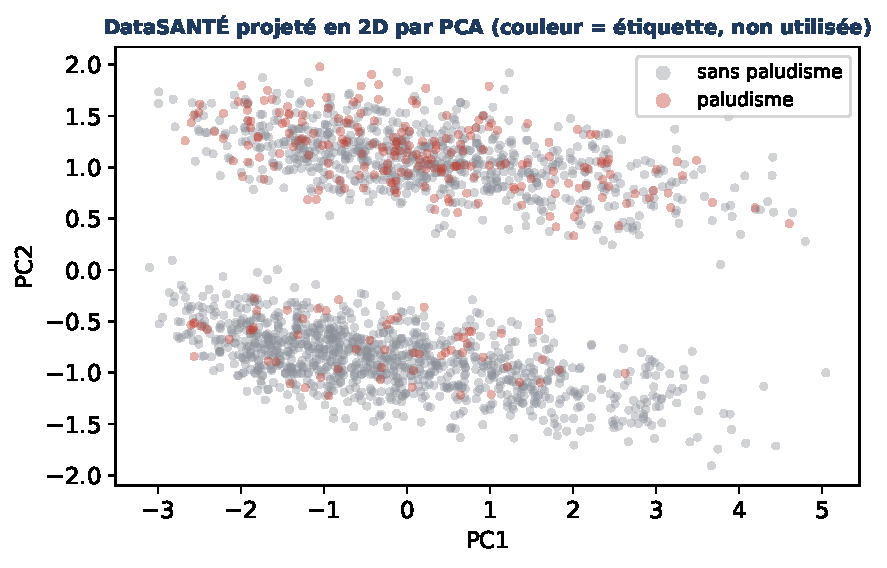
\includegraphics[width=0.44\linewidth,height=0.40\textheight,keepaspectratio]{f9_pca_datasante}\end{center}

{\scriptsize Chaque point est un patient (PC1–PC2). La couleur (rouge = paludisme) \emph{n'a pas servi} à la projection : on devine pourtant un gradient — la PCA, sans étiquette, organise déjà les patients d'une façon liée à la maladie.}
\end{frame}

\begin{frame}{Piège — la PCA exige la standardisation et reste linéaire}
\begin{ucadpiege}[Deux limites à connaître]
{\small \textbf{(1) Standardisation} : la PCA maximise la variance ; sans standardisation, une variable à grande échelle accapare les premières composantes, comme pour k-means. Toujours standardiser avant. \textbf{(2) Linéarité} : la PCA ne capte que des directions \emph{droites} de variance ; une structure courbe ou non-linéaire lui échappe.}
\end{ucadpiege}
{\small Autre limite : les composantes principales sont des \emph{combinaisons} des variables d'origine, souvent difficiles à interpréter (« $0{,}4 \times$ âge $- 0{,}3 \times$ glycémie $+ \dots$ »). La PCA est excellente pour compresser, visualiser et débruiter, mais elle sacrifie l'interprétabilité directe des variables. Comme toujours, un outil puissant a son revers : ici, la lisibilité.}
\end{frame}

\begin{frame}[fragile]{En pratique : PCA}
\begin{lstlisting}
from sklearn.preprocessing import StandardScaler
from sklearn.decomposition import PCA

X = StandardScaler().fit_transform(df[colonnes])   # OBLIGATOIRE
pca = PCA(n_components=2)        # garder 2 composantes
X_reduit = pca.fit_transform(X) # les donnees en 2D

print(pca.explained_variance_ratio_)        # variance par composante
print(pca.explained_variance_ratio_.sum())  # variance totale conservee
\end{lstlisting}
{\small \texttt{n\_components=2} demande deux composantes (pour visualiser) ; on peut aussi passer un seuil, par exemple \texttt{PCA(n\_components=0.8)} pour garder automatiquement assez de composantes pour $80\,\%$ de variance. \texttt{explained\_variance\_ratio\_} donne la part de variance de chaque composante — le critère de choix. Standardiser avant reste impératif.}
\end{frame}

% #####################################################################
\section{Application : la structure cachée de DataSANTÉ}

\begin{frame}{Le mini-défi : le clustering connaît-il le paludisme ?}
\begin{ucadfront}[Une question révélatrice]
{\small Test décisif du non-supervisé : on lance k-means sur les patients de DataSANTÉ \emph{sans jamais lui montrer l'étiquette paludisme}. Question : les clusters qu'il forme ont-ils un lien avec la maladie ? Si oui, c'est la preuve que la structure non-supervisée capte quelque chose de réel — alors qu'aucune réponse ne lui a été donnée.}
\end{ucadfront}
{\small On standardise cinq variables (âge, glycémie, hémoglobine, fièvre, saison), on demande $k = 3$ clusters, puis — \emph{seulement après} — on regarde le taux de paludisme dans chaque cluster. Le clustering n'a aucune information sur la maladie ; tout lien observé émerge de la seule structure des données.}
\end{frame}

\begin{frame}{Le verdict : des groupes de risque très différents}
\figslide{0.64}{f9_cluster_palu}{Sans voir l'étiquette, k-means forme trois groupes aux taux de paludisme \emph{très} différents : cluster « pluies » ($100\,\%$) avec $\mathbf{20{,}5\,\%}$ de paludisme, contre cluster « sec » ($0\,\%$) à $\mathbf{5{,}2\,\%}$ (global $11{,}8\,\%$). Le clustering a retrouvé, seul, un facteur de risque majeur.}
\end{frame}

\begin{frame}{La leçon de l'application}
\begin{ucadret}[Le non-supervisé révèle du réel]
{\small Le fait marquant : un algorithme à qui l'on n'a donné \emph{aucune} étiquette retrouve une structure liée au diagnostic. Cela montre que les regroupements ne sont pas arbitraires — ils reflètent des profils cliniques réels. C'est toute la valeur du non-supervisé : faire émerger des structures \emph{avant} toute annotation, parfois là où on ne les attendait pas.}
\end{ucadret}
{\small Usages concrets : segmenter une patientèle pour adapter la prise en charge, repérer des profils atypiques (détection d'anomalies), ou explorer un jeu de données neuf pour orienter les analyses suivantes. Le non-supervisé est souvent la \emph{première} étape d'un projet — comprendre la structure — avant de passer, si besoin, au supervisé.}
\end{frame}

% #####################################################################
\section{Synthèse}

\begin{frame}{Clustering et réduction : deux usages distincts}
\begin{ucadret}[Quand utiliser quoi]
{\small \begin{center}\renewcommand{\arraystretch}{1.25}
\begin{tabular}{l|l}
\textbf{besoin} & \textbf{outil}\\\hline
regrouper des exemples similaires & clustering (k-means)\\
segmenter une patientèle, des profils & clustering (k-means)\\
visualiser des données à $>2$ variables & PCA (2 composantes)\\
compresser / débruiter avant un modèle & PCA (seuil de variance)\\
détecter des structures inconnues & clustering puis PCA\\
\end{tabular}\end{center}}
\end{ucadret}
\end{frame}

\begin{frame}{Le protocole non-supervisé}
\begin{ucadret}[De bout en bout]
{\small \textbf{1.} \textbf{Standardiser} les variables (impératif pour la distance comme pour la variance) $\to$ \textbf{2.} pour \emph{regrouper} : k-means avec \texttt{n\_init} élevé, choisir $k$ par le coude \emph{et} la silhouette $\to$ \textbf{3.} pour \emph{réduire} : PCA, choisir le nombre de composantes par la variance cumulée (seuil $80$–$90\,\%$) $\to$ \textbf{4.} \emph{interpréter} les clusters ou les composantes au regard du métier $\to$ \textbf{5.} se rappeler les limites : k-means suppose des clusters ronds, la PCA est linéaire. En cas de structure complexe, envisager d'autres méthodes.}
\end{ucadret}
\end{frame}

\begin{frame}{À retenir — Séance 9 (1/2)}
\begin{ucadret}[Le clustering]
\begin{itemize}\small
  \item Le \textbf{non-supervisé} cherche une structure \emph{sans étiquettes} : regrouper (clustering) ou simplifier (réduction de dimension).
  \item \textbf{k-means} alterne \emph{affectation} (chaque point au centre le plus proche) et \emph{mise à jour} (chaque centre $=$ moyenne de ses points), jusqu'à convergence.
  \item Il minimise l'\textbf{inertie} (compacité des clusters) ; il converge vers un \emph{minimum local} — d'où \texttt{n\_init} élevé.
  \item Choisir $k$ : la \textbf{méthode du coude} (inertie) et le \textbf{score de silhouette} (maximiser). Toujours \textbf{standardiser} ; attention aux clusters non sphériques.
\end{itemize}
\end{ucadret}
\end{frame}

\begin{frame}{À retenir — Séance 9 (2/2)}
\begin{ucadret}[La réduction de dimension]
\begin{itemize}\small
  \item Fondations : \textbf{variance} (étalement), \textbf{covariance} (variation conjointe), \textbf{vecteurs propres} ($A\mathbf{v} = \lambda\mathbf{v}$, les axes d'une matrice).
  \item La \textbf{PCA} projette les données sur les directions de variance maximale (vecteurs propres de la covariance) ; les valeurs propres mesurent la variance captée.
  \item Choisir le nombre de composantes par la \textbf{variance cumulée} (seuil $80$–$90\,\%$). Sur DataSANTÉ : $4$ composantes pour $80\,\%$.
  \item Limites : \textbf{standardiser} d'abord ; la PCA est \emph{linéaire} et ses composantes sont peu interprétables.
\end{itemize}
\end{ucadret}
\end{frame}

\begin{frame}{Pièges fréquents}
\begin{itemize}\small
  \item Oublier de \textbf{standardiser} : les variables à grande échelle dominent la distance (k-means) et la variance (PCA).
  \item Lancer k-means une seule fois : risque de tomber sur un mauvais minimum local — utiliser \texttt{n\_init}.
  \item Choisir $k$ au hasard : croiser le coude, la silhouette et le bon sens métier.
  \item Appliquer k-means à des clusters non sphériques (lunes, anneaux) : il échouera.
  \item Garder trop peu de composantes en PCA : vérifier la variance cumulée avant de réduire.
  \item Interpréter les composantes principales comme des variables d'origine : ce sont des combinaisons, souvent opaques.
\end{itemize}
\end{frame}

\begin{frame}{Prochaine séance}
\begin{ucadfront}[Séance 10 — Les réseaux de neurones]
{\small Retour au supervisé, mais avec le modèle le plus emblématique de l'IA moderne : le \textbf{réseau de neurones}. On verra que sa brique de base est la régression logistique de la Séance 6, comment empiler des couches, et — pour les curieux — comment un réseau apprend par rétropropagation. Et l'on posera la question honnête : sur nos données, bat-il vraiment les méthodes d'ensemble de la Séance 8 ?}
\end{ucadfront}
\end{frame}

\begin{frame}{Références}
\begin{itemize}\small
  \item Géron — \emph{Hands-On Machine Learning}, 3\textsuperscript{e} éd., O'Reilly, 2022 (clustering, réduction de dimension).
  \item Müller, Guido — \emph{Introduction to Machine Learning with Python}, O'Reilly, 2016.
  \item James, Witten, Hastie, Tibshirani — \emph{An Introduction to Statistical Learning}, 2\textsuperscript{e} éd., Springer, 2021 (chap. 12).
  \item Hastie, Tibshirani, Friedman — \emph{The Elements of Statistical Learning}, Springer, 2009.
  \item Cours : University of Washington CSE 446 ; Stanford CS229 (apprentissage non-supervisé).
\end{itemize}
\end{frame}

\end{document}
